\documentclass{scsSimAUDPaperFormat}
% Beginning of preable.
% Ensure that the copyright notice matches the conference/symposium.
\copyrightnotice{
	SimAUD 2020 May 25-27 Vienna, Austria
	
	\copyright\,2020 Society for Modeling \& Simulation International (SCS)
}
% Load basic packages
\usepackage{balance}		% to better equalize the last page
\usepackage{graphics}		% for EPS, load graphicx instead
\usepackage{times}			% comment if you want LaTeX's default font
\usepackage{url}			% llt: nicely formatted URLs
\usepackage{dblfloatfix}	% allow placement of a page-width figure at top or bottom of page
% llt: Define a global style for URLs, rather that the default one

\usepackage{listings}
\lstdefinestyle{mystyle}{
    %backgroundcolor=\color{backcolour},   
    %commentstyle=\color{codegreen},
    keywordstyle=\color{magenta},
    %numberstyle=\tiny\color{codegray},
    %stringstyle=\color{codepurple},
    basicstyle=\ttfamily\footnotesize,
    breakatwhitespace=false,         
    breaklines=true,                 
    captionpos=b,                    
    keepspaces=true,                 
    numbers=left,                    
    numbersep=5pt,                  
    showspaces=false,                
    showstringspaces=false,
    showtabs=false,                  
    tabsize=2
}
 
\lstset{style=mystyle}

\makeatletter
\def\url@leostyle{%
  \@ifundefined{selectfont}{\def\UrlFont{\sf}}{\def\UrlFont{\small\bf\ttfamily}}}
\makeatother
\urlstyle{leo}

% To make various LaTeX processors do the right thing with page size.
\def\pprw{8.5in}
\def\pprh{11in}
\special{papersize=\pprw,\pprh}
\setlength{\paperwidth}{\pprw}
\setlength{\paperheight}{\pprh}
\setlength{\pdfpagewidth}{\pprw}
\setlength{\pdfpageheight}{\pprh}

% Make sure hyperref comes last of your loaded packages,
% to give it a fighting chance of not being over-written,
% since its job is to redefine many LaTeX commands.
\usepackage[pdftex]{hyperref}
\hypersetup{
pdftitle={SCS Conference Proceedings Format},
pdfauthor={LaTeX},
pdfkeywords={SCS, proceedings, archival format},
bookmarksnumbered,
pdfstartview={FitH},
colorlinks,
citecolor=black,
filecolor=black,
linkcolor=black,
urlcolor=black,
breaklinks=true,
}

% create a shortcut to typeset table headings
\newcommand\tabhead[1]{\small\textbf{#1}}

% create an affilitation superscript
\newcommand{\affiliation}[1]{\ensuremath{^{\textrm{#1}}}}

% End of preamble. Here comes the document.

\begin{document}
\title{
\includegraphics[width=1.0\textwidth]{SimAUDLogo.png}\\\quad\\Modeling and Simulation of Municipal Solid Waste Management System based on Discrete Event System Specification}

% Replace "UniversityA", "CompanyA", "UniversityB" with institution-specific abbreviations.
\def\UniversityA{\affiliation{1}} 
\def\CompanyA{\affiliation{2}}

\author{
	Chang-Hyun Lyoo\UniversityA
	,
	Jinho Jeong\UniversityA
	,
	Changbeom Choi\UniversityA
	\,and
	Eun-Young Kim\CompanyA
	\\
	\\
\affaddr{\UniversityA}{Handong Global University, Pohang, Rep. of Korea, \{21300259, 21300704, cbchoi\}@handong.edu}\\
\affaddr{\CompanyA}{Pohang TechnoPark, Pohang, Rep. of Korea, hellosally@daum.net}
}

\maketitle

\begin{abstract}
%생활쓰레기수거는 시민들의 편의에 큰 영향을 미치는 중요한 도시행정서비스이다. 
 Cleanliness of garbage house and garbage collection affects residential satisfaction. Proper solid waste management system is required for citizen's life and convenience.
 In this paper, we focus on the temporal behavior pattern of residents in the area.
 
 !!!about experimental design and the method!!!
 ??We use Discrete Event System Specification? for simulation


\end{abstract}

\keywords{
	Agent-based Simulation; Discrete Event Sytem Formalism; Municipal Solid waste Management System.
\\
}

% ACM Classification Keywords
\category{I.6.5} \
SIMULATION AND MODELING (Model Development).
\\

\section{Introduction}
Today, 55\% of the world’s population lives in urban areas, a proportion that is expected to increase to 68\% by 2050.~\cite{united20182018} Urbanization continues and population is steadily increasing.As being more populated, total amount of garbage within local area is increasing.
The garbage problem is closely related to satisfaction of citizens among many urban issues\cite{mohit2010assessment}.
Therefore, solid waste collection is becoming important and it affects citizen’s satisfaction and convenience. If garbage is not collected well than people become unsatisfied then even file a civil complaint. This will lead to waste of administrative power and increase social cost. 


Some work has been done to optimize the route of the garbage truck and reduce waste collecting costs using agent based simulation and GIS\cite{dyson2005forecasting}\cite{}. Most of simulation studies for waste management have been carried out using GIS.



However, as far as the authors know, there are no research built human pattern model considering culture, characteristics of residents and the degree of development. Human behavior pattern is important factor rather than geographic or demographic characteristics of urban.
In this study, we propose a model focusing on human characteristics and behavior pattern to optimize MSW management system. By doing so, we can figure out which waste collection policy would fit and increase the overall satisfaction of citizens. 

The result of simulation demonstrate satisfaction level of the citizens and number of filed complaints.

%DEVS formalism 에 대한 이야기 
Since the behavior of the residents may differ based on their life cycle and occupation, this research utilizes the Discrete Event System(DEVS) formalism to model the behavior of the residents. The DEVS formalism
is a set-theoretical framework and has a modular characteristic~\cite{Zeigler84, Zeigler90, tms2000}. As a result,the simulationists may develop their simulation model as a component of the urban system or may reuse a different simulation model which is built by other simulationists. 
To maximize the modular characteristic of the DEVS Formalism, this research proposes an object-oriented discrete event simulator using the Python programming language. The simulator captures the default behavior of the residents of the urban area using DEVS Formalism and specializes the residents by their occupation. Therefore, simulationists may reuse the DEVS simulation model to simulation the temporal behavior of the residents and may differentiate each resident by using occupation object. 

\section{Related Works and Backgrounds}
This section introduces the related works and analyze them. Also, it provides the background knowledge to understand the proposed method and the simulation environment.

\subsection{Related Works: Waste Managements}
There have been many studies to optimize the waste management applying computer programming GIS analysis, simulation models, system dynamics, integer linear programming(ILP), and mixed integer linear programming(MILP).
Karadmias et al(2006)\cite{karadimas2006coupling} integrated GIS analysis and agent based simulation
et al 
\cite{karadimas2006coupling} focused on integration of GIS and multi agent simulation system. 
Agent-based simulation and GIS applied waste management system optimizations are proposed in the literature. \cite{karadimas2006coupling,shi2013multi,nguyenemission,nambiar2013multi,hua2016towards}

There are many studies using GIS and Agent based simulations to optimize waste management system.


% Please add the following required packages to your document preamble:
 %\usepackage{booktabs}
%\begin{table}[]
%\begin{tabular}{lllllll}
%Property & GIS & AGENT & DISCRETE & ROUTING & DECISION SUPPORT & SYSTEM DYNAMICS \\
%Shi, X., Thanos, A. E., \& Celik, N. (2014) & X & O & Hybrid & X & FRAMEWORK &  \\
%Shi, X., Thanos, A. E., \& Antmann, E. D. (2013). & O & O & Hybrid & O &  &  \\
%Guariso, G., Michetti, F., Porta, F., \& Moore, S. (2009). & X & X & O & X & X & O \\
%Antmann, E. D., Shi, X., Celik, N., \& Dai, Y. (2013). & X & X & O & X & O & X \\
%Meng, X., Wen, Z., \& Qian, Y. (2018). & X & O & X & X & O & X \\
%Dyson, B., \& Chang, N. B. (2005). & X & X & X & X & X & O \\
%Wang, C. (2017, May). & X & X & X & X & X & O \\
%Karadimas, N. V., Rigopoulos, G., \& Bardis, N. (2006). & O & O & X & X & X & X \\
%Nguyen-Trong, K., Dinh-Thi-Hai, V., Nguyen-Thi-Ngoc, A., \& Nguyen-Ngoc, D.(2017). & O & O & X & O & X & X \\
%Nambiar, S. K., \& Idicula, S. M. (2013, December). & O & O & X & O & X & X \\
%Hua, T. M., Nguyen, T. K., Van Dinh Thi, H., \& Thi, N. A. N. (2016, December). & O & O & X & O & X & X \\
%Das, S., \& Bhattacharyya, B. K. (2015). & O & X & X & O & X & X \\
%Chalkias, C., \& Lasaridi, K. (2009). & O & X & X & O & X & X \\
%Dao-Tuan, A., Nguyen-Thi-Ngoc, A., Nguyen-Trong, K., Bui-Tuan, A., \& Dinh-Thi-Hai, V. (2017, September). & O & X & X & O & X & X \\
%Dennison, G. J., Dodd, V. A., \& Whelan, B. (1996). & X & X & X & X & X & X
%\end{tabular}
%\end{table}

%쓰레기 수집 자체 과정에 있어서 쓰레기차의 경로 설정 문제를 다양한 방법들로 해결 한 경우도 있었고,
%쓰레기 수거 및 후처리 시스템 까지 전반적인 시스템을 시뮬레이션한 논문도 있었으나
%특별히 거주민들의 시간적 패턴을 가지고 만족도를 분석한 모델은 존재 하지 않았다.
%그런점에서 우리의 연구는 참신하고 GIS 데이터를 이용하여 단순히 인구를 기준으로 쓰레기의ㅏ 양을 예측하는 %것이 아니라 사람들의 쓰레기 배출 패턴을 시뮬레이션 함으로써 좀더 정확하게 만족도 측정이 가능해졌다.
%다음 연구들의 한계점은 다음과 같다. 
%다른사람이 연구한 방법들에 대해서 소개
%제한점들	ex)문화에 대한 고려가 없었다

\subsection{Backgrounds: Discrete Event System Specification}
The DEVS formalism is a set-theoretic formalism developed for specifying discrete event systems. The DEVS formalism has two models to represent a discrete event system, the $Atomic Model$ and the $Coupled Model$. 
The simulationist may specify the behavior of a component of the discrete event system using an atomic model and assembles the Atomic Models to build a bigger system using a Coupled Model. This research adopts the specification of the Atomic Model to represent the behavior of the participant simulation models of the urban simulation. The specification of the Atomic Model is defined as follows.

An Atomic Model is defined as follow:
\begin{tabbing}
xxxx\=xxxx\=xxxx\=xxxx\=\kill\\
\> \> \> $AM$ = $<X, Y, S, \delta_{ext}, \delta_{int}, \lambda, ta>$\\
where\\
\> $X$: a set of external input event types,\\
\> $Y$: an output set,\\
\> $S$: a sequential state set,\\
\> $\delta_{ext}$: $Q \times X \rightarrow S$, an external transition function\\
\> \> where $Q$ is the total state set of \\
\> \> $M$ = $\{(s,e)|s \in S\:and\:0 \leq e \leq ta(s)\}$,\\
\> $\delta_{int}$: $S \rightarrow S$, an internal transition function,\\
\> $\lambda$: $S \rightarrow Y$, an output function,\\
\> $ta$: $S \rightarrow {\cal R}^{+}_{0,\infty}$, a time advance function, \\
\> \> where the ${\cal R}^{+}_{0,\infty}$ is the non-negative real numbers \\
\> \> with $\infty$ adjoined.
\end{tabbing}

An atomic model $AM$ is a model which is affected by external input events
$X$ and which in turn generates output events $Y$.
The state set $S$ represents the unique description of the model.
The internal transition function $\delta_{int}$ and the external transition
function $\delta_{ext}$ compute the next state of the model.
If an external event arrives at the elapsed time $e$ which is less than or
equal to $ta(s)$ specified by the time advance function $ta$, a new
state $s'$ is computed by the external transition function $\delta_{ext}$.
Then, a new $ta(s')$ is computed, and the elapsed time $e$ is set to zero.
Otherwise, an internal event arrives at $ta(s)$, and then a new state
$s'$ is computed by the internal transition function $\delta_{int}$.
In the case of internal events, the output specified by the output function
$\lambda$ is produced based on the state $s$, which means the output function
is processed before the internal transition function.
Then, as before, a new $ta(s')$ is computed, and the elapsed time $e$ is set to zero. 

\begin{figure}[!h]
    \centering
    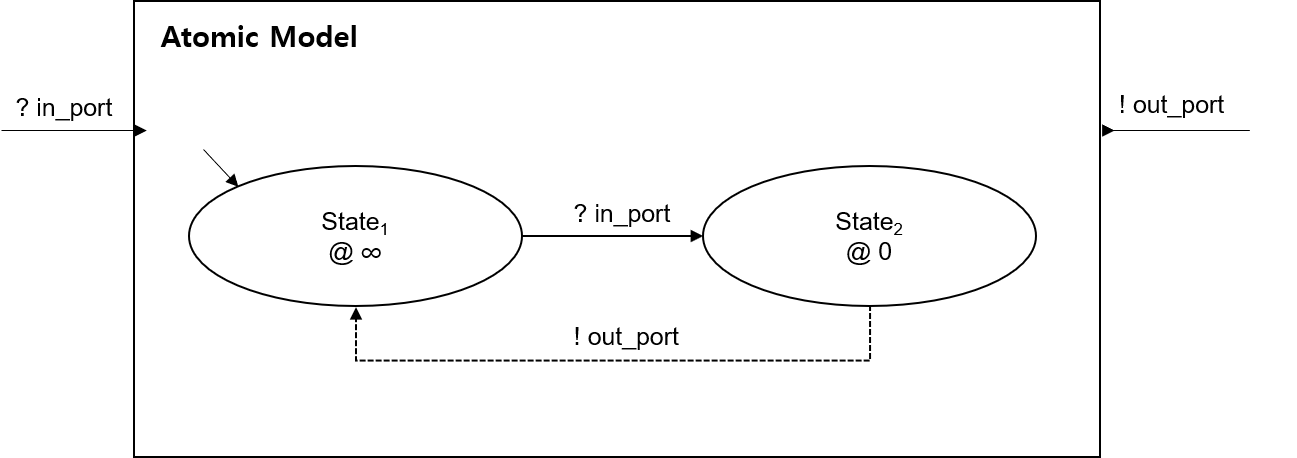
\includegraphics[width=1.0\columnwidth]{fig/Atomic_model}
    \caption{Example of an Atomic Model}
    \label{Fig:AtomicModel}
\end{figure}

Fig.~\ref{Fig:AtomicModel} shows the diagram of an Atomic Model. The label starting with the question mark denotes the input port, and the label starting with the bang denotes the output port. The ellipse shows the state of the model and ellipse with arrow denotes the initial state of the model. Each state has the state name and the positive real number which denotes the occupancy time. When the elapsed time meets the occupancy time, the simulation algorithm will trigger the output function and internal transition function, sequentially. 

The proposed simulator partially accepts the notation of DEVS Formalism and its simulation algorithm. Listing~\ref{lst:atomic} shows the python code of the example atomic model. As shown in the Listing~\ref{lst:atomic}, the proposed simulator provides a programming interface that has a one-to-one correspondence with the Atomic Model specification of the DEVS formalism.


\begin{lstlisting}[language=Python, caption=Example Code of Atomic Model, label={lst:atomic}]
class AtomicModel(BehaviorModelExecutor):
    def __init__(self, instance_time, destruct_time, name, engine_name):
        BehaviorModelExecutor.__init__(self, instance_time, destruct_time, name, engine_name)

        self.init_state("State1")
        self.insert_state("State1", Infinite)
        self.insert_state("State2", 0)

        self.insert_input_port("in_port")
        self.insert_output_port("out_port")

    def ext_trans(self,port, msg):
        if port == "in_port":
            self._cur_state = "State2"

    def output(self):
        name = self.get_name()
        msg = SysMessage(name, "out_port")
        return msg
        
    def int_trans(self):
        if self._cur_state == "State2":
            self._cur_state = "State1"
\end{lstlisting}

\section{Proposed Method and Environments}

This section introduces the proposed method to model the municipal solid waste management system and its simulation environment. To capture the dynamic behavior of the residents, we classified the type of the residents and model them in the object-oriented fashion. After modeling the resident, we developed a simulation model to represent the housing type. Finally, we developed simulation models to provide municipal solid waste management services to the residents. 

\subsection{Modeling of an Urban Waste Management System}
To model the residential area. 
\begin{figure}[!h]
    \centering
    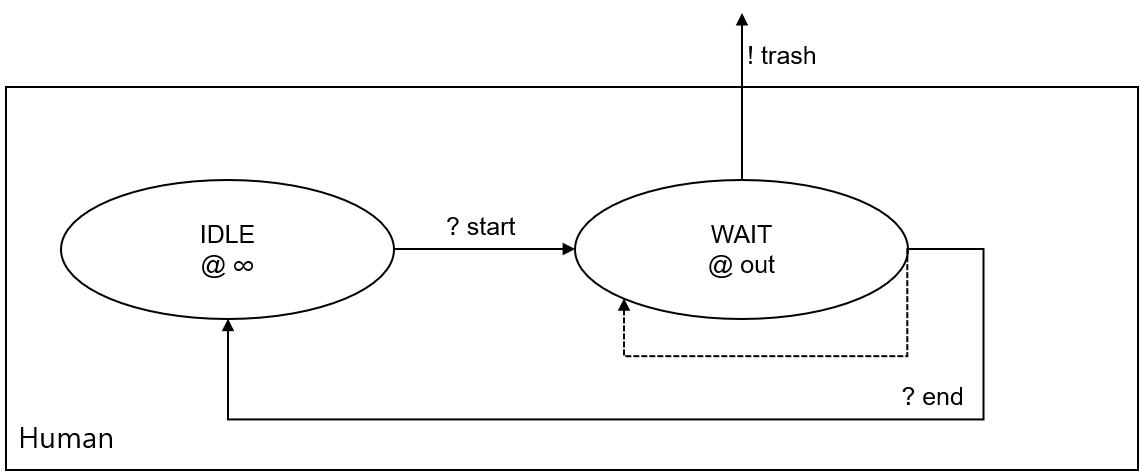
\includegraphics[width=1.0\columnwidth]{fig/human_model.png}
    \caption{Atomic Model of a Resident}
    \label{Fig:Humanmodel}
\end{figure}

\begin{figure}[!h]
    \centering
    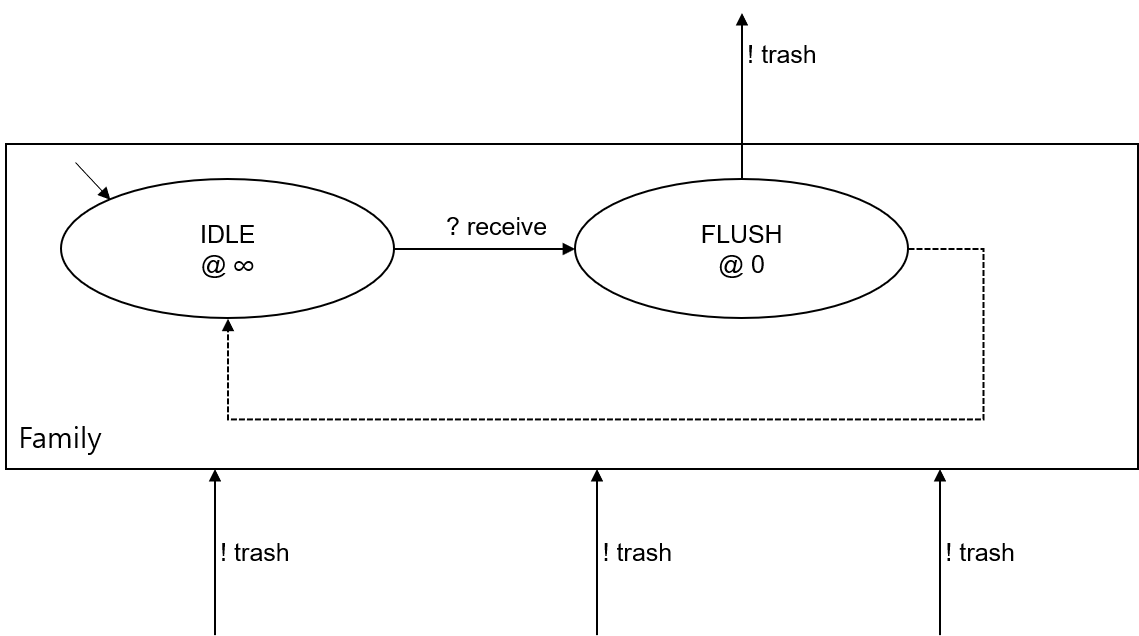
\includegraphics[width=1.0\columnwidth]{fig/family_model.png}
    \caption{Atomic Model of a Housing Type}
    \label{Fig:Familymodel}
\end{figure}

\begin{figure}[!h]
    \centering
    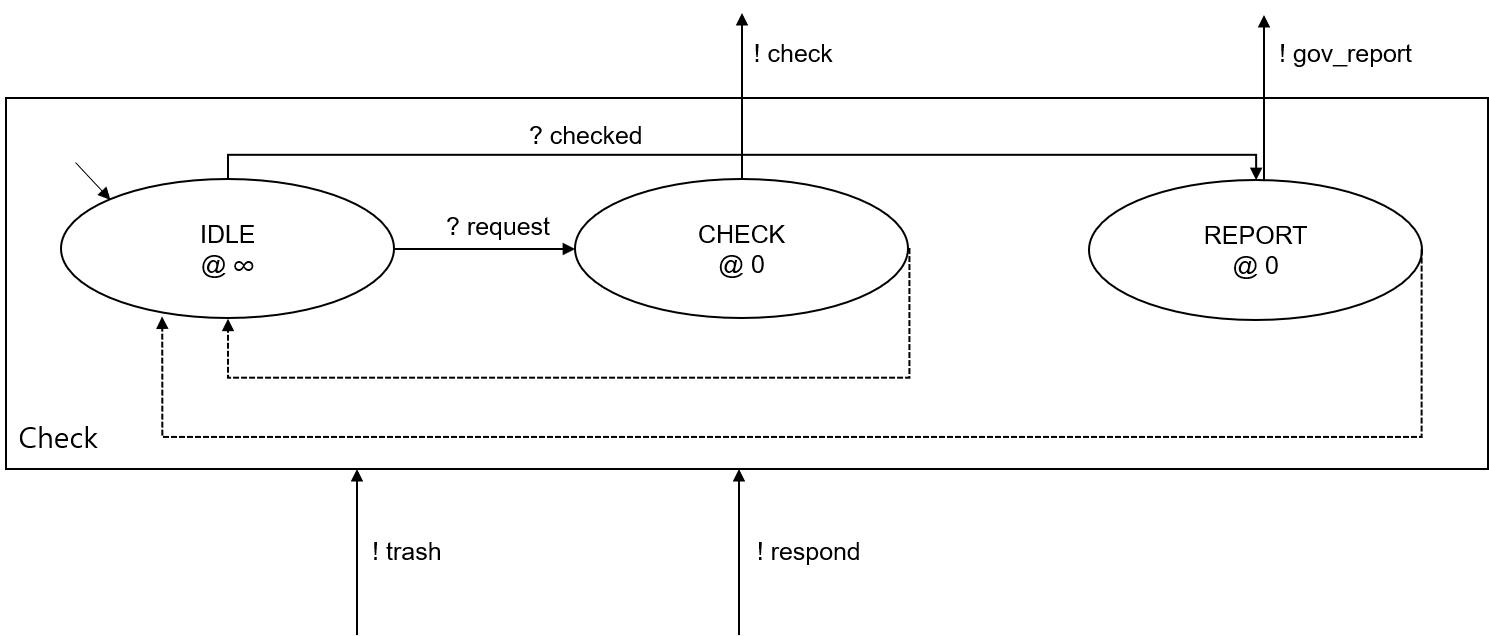
\includegraphics[width=1.0\columnwidth]{fig/check_model.png}
    \caption{Atomic Model to Calculate the Satisfaction Level of a Resident}
    \label{Fig:Checkmodel}
\end{figure}

\begin{figure}[!h]
    \centering
    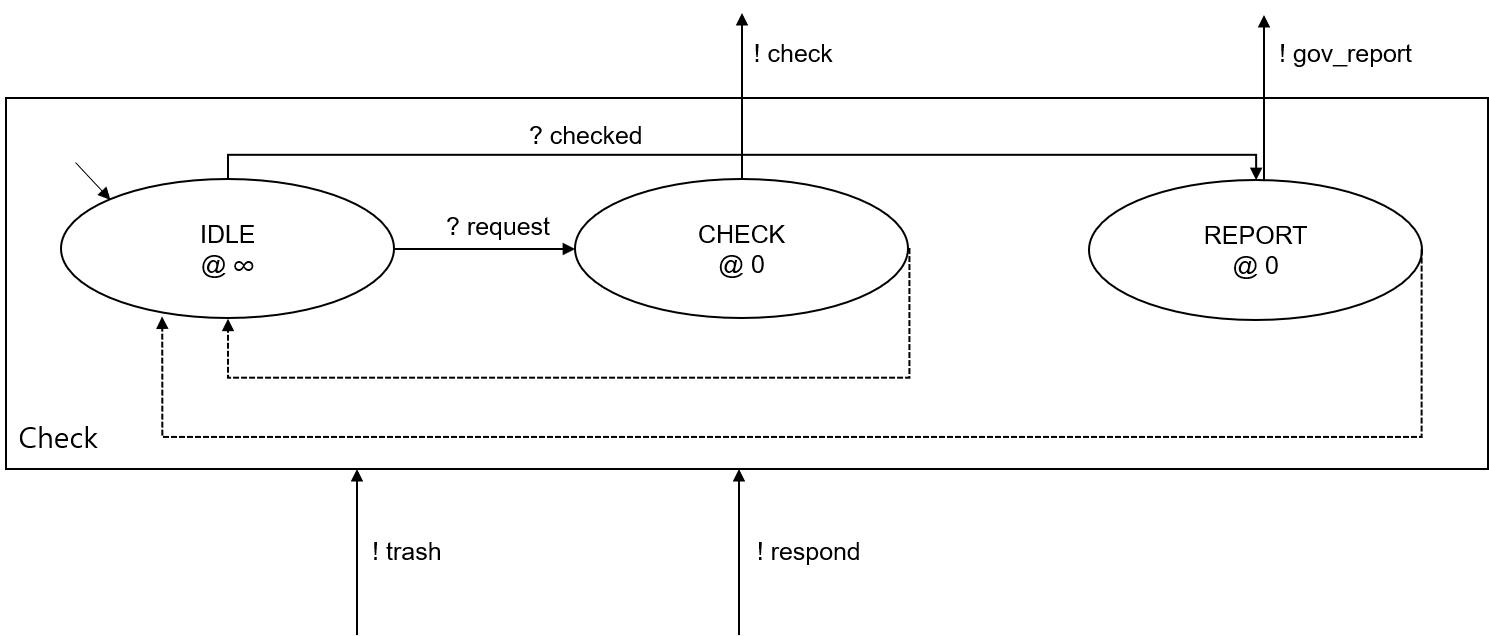
\includegraphics[width=1.0\columnwidth]{fig/check_model.png}
    \caption{Diagram of an Atomic Model}
    \label{Fig:Checkmodel}
\end{figure}
% 모델링을 어떻게 했다. 
% 사람, 직업, 행위에 대해서 모델링을 어떻게 했다고 작성




%우리가 하려는 것들
%Behaviourmodel, Familymodel, garbagecan, garbagetruck, checker 등등 
%상속 하는 그림,
%각 모델에서 설명 (human - 직업)
%직업이 simulation에 영향을 줌 -> 직업별 행동패턴을 부여해서 모델링 하는게 좋다
%Report하는 사람과 안하는 사람 리스트나 튜플 형태로 표현



\subsection{Simulation Environments}
%개발한 시뮬레이터 코드 설명 %교수님
%Diagram, 코드설명 같이


Explanation about evsim

\section{Case Study}
This section illustrates the case study of the proposed method and the simulation environments. This research models the Jang-Ryang district of the Pohang city in the Republic of Korea. The composition of the residents in Jang-Ryang district is different than other residential area. There are two colleges and one university located nearby, so many students live in a studio apartment complex during the school year. Also, the portion of the construction workers grows and subsides due to the construction plan of the city. The behaviors of the college students and the construction workers are different. 

\subsection{Assumptions and the Simulation Parameters}
Followings are the assumptions to model the Jang-Ryang district.
\begin{itemize}
    \item Each building has a garbage can to hold the garbage temporally.
    \item Each resident has their own schedule to go out.
    \item Every resident emits garbage every day when they go out. 
    \item If residents have a family, then they emit garbage as a family together.
    \item The garbage truck collects the garbage from the building regularly.
    \item The satisfaction level of the resident may change at the moment when resident emits the garbage.
    \item The resident may claim to the Government when the garbage goes above a certain level.
\end{itemize}

Following Table~\ref{tab:SimParam} shows the simulation parameters deduced from the assumptions.

%As of February 2019, 71,802 people are currently residing in this area.
%Pohang city, the Republic of Korea began to develop after Pohang Iron and Steel Company was established in 1968. Jangryang district was only a remote village with a population of more than 1,900 in 1981. In the early 2000s, many apartments were built and a bed town was formed under the city development plan. The population began to move in as long-range housing districts were formed. The largest population in Pohang has been living in Jangryang-dong since 2011. As of February 2019, 71,802 people are currently residing in this area. The ratio of blue collars is high as the industrial complex's full-fledged operation brings in the population. Since convenient traffic conditions and commercial districts are easy to bring in tenants, most of the real-life residents are short-term residents. Also, there are two colleges and one university located nearby, so many students live in a studio apartment complex during the school year. 

%The prediction of municipal solid waste generation plays an important role in a solid waste management.

\begin{table*}[ht]
\centering
\caption{Description of Simulation Parameters}
\begin{tabular}{|l|c|c|}
\hline
 & Construction Workers & Student \\ \hline
Leave Time & 6:22:00 & 7:58:00 \\ \hline
Amount of Waste Emission & 0.9 & 0.9 \\ \hline
Satisfaction Function & 
    $Satis(x) = \begin{cases}
              + 10 & \text{if } x < 0.8,\\
              \ \ \ 20 & \text{if } x = 0,\\
               -10 & \text{if } x > 0.8
          \end{cases}$
 & $Satis(x) = \begin{cases}
              + 10 & \text{if } x < 0.8,\\
              \ \ \ 20 & \text{if } x = 0,\\
               -10 & \text{if } x > 0.8
          \end{cases}$ \\ \hline
\end{tabular}
\label{tab:SimParam}
\end{table*}

$Out\_time$ parameter represent an interval at which one leaves one's home, and the $trash$ parameter represents the amount of waste generated until out time. For realistic simulation, the trash generation amount of residents drawn from average waste emissions per capita.\cite{Korea_resource_recirculation_information_system_2018}. $satisfaction$ parameter represents one's satisfaction level according to the level of garbage. Based on the experiences of some students, the decision made by the heuristic.

%out_time?


% 이상의 파라미터 값이 어떻게 책정되었는지가 설명되어야 함

\begin{figure}[!h]
    \centering
    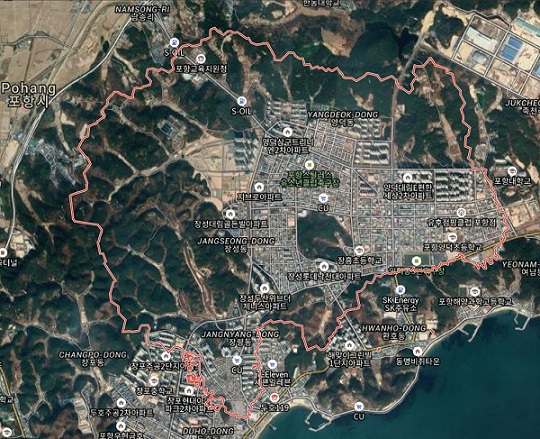
\includegraphics[width=1.0\columnwidth]{fig/map.jpg}
    \caption{Map of Jangryang-dong, Pohang represented within the red bold lines}
    \label{Fig:JangYrang}
\end{figure}

%조사한 내용 설명 -> 코드에 어떻게 들어가는지
%Graph그리기

\\
%%이루어지지 않고있다.장량동은 인구 7만3000명이 거주하는 포항에서 가장 큰 행정동으로 타 지역에 비해 평균연령이 상대적으로 낮고, 학생이 차지하는 비율이 높다. 또한, 포항은 철강산업단지의 본격적인 가동으로 공단 인구가 유입됨에따라 Blue collar의 비율이 높다. 비교적 편리한 교통여건과 상권이 형성돼 세입자를 들이기 쉬운 여건이어서 대표적인 원룸촌이 형성돼 있어 실거주자의 대부분이 단기 거주자인 특징을 가지고 있다. 
%이번 연구에서는 대한민국 포항에 새롭게 형성된 신도시 양덕동 주변의 원룸촌을 모델링 대상으로 설정하였다
\subsection{Jang-Ryang District Model and Simulation Results}

\begin{figure}[!h]
    \centering
    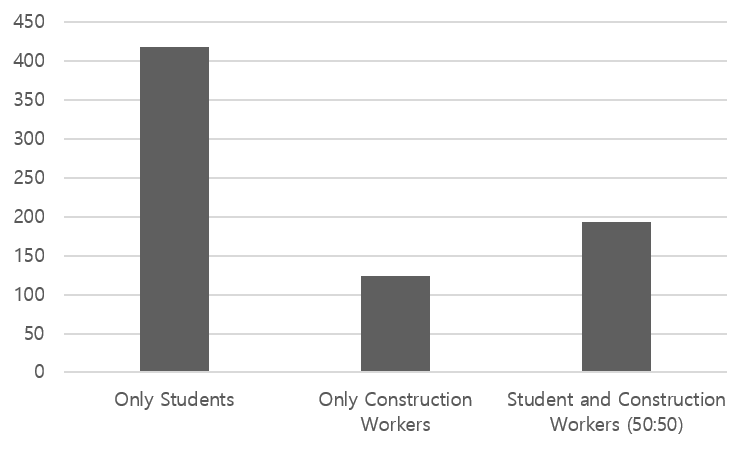
\includegraphics[width=1.0\columnwidth]{fig/case_study_result.png}
    \caption{Number of complaints according to the percentage of resident occupations}
    \label{Fig:case_result}
\end{figure}

\section{Conclusion}
%우리의 모델은 훌륭했다. 하지만 UI 적으로 공무원들이나 일반인들이 사용하기에는 무리가 있을것으로 예상된다. 이 부분을 보완해서 나중에 FLASK등과 연결하여 쉬운 인터페이스로 작동하도록 하면 좋을 것 같다.


\balance

\bibliographystyle{scsBiblioStyle}
\bibliography{SampleReferences}

\end{document}
